%&latex
%
\providecommand{\main}{../..}
\documentclass[../../main.tex]{subfiles}
\usepackage{amssymb}

\begin{document}

\section{Critical Behaviours and Scaling Laws}
\lesson{22}{29/04/20}

In the last section, we were able to finally describe a \textbf{phase-transition} , by analysing the Ising Model in the mean field approximation in $d > 1$. Mathematically, we observed how the \textbf{spontaneous magnetization} $M(K, h)$,\marginpar{Power laws} when $K$ is chosen in the proximity of the \textit{critical parameter} $K_c$ needed for the phase-transition, is described by a \textbf{power law} (\ref{eqn:mean-field-MS}).

\medskip

This happens to be a very general kind of behaviour, proper of \textbf{not only} \textbf{mean field} models.
Scaling laws such as (\ref{eqn:mean-field-MS}) were originally formulated from empirical evidence, and then given a theoretical foundation in the 1960s by Widom, Kadanoff and Kenneth Wilson, leading to the field of \textbf{renormalization group theory}. In this framework, all critical phenomena can be treated on equal ground, and general results can be mathematically proven. 

\medskip

The importance of scaling laws, and especially the values of their \textit{critical exponents} (such as $\beta$ for the IM) resides in their \textbf{universality}, i.e. in the fact that they are \textit{largely independent} on the \q{model's details}. In other words, the very same scaling law can describe two systems that - from the outside - seem completely different - but that share some fundamental characteristic (e.g. symmetry). 

\medskip

So, let's continue using the Ising Model in the mean field approximation as a \textit{concrete} example, and let's focus on deriving and understanding scaling laws for various quantities of interest.

\subsection{Spontaneous magnetization}
We start with (re)deriving the power law for the \textbf{spontaneous magnetization}. Recall the expression for the variational free energy (\ref{eqn:FV-uniform}):
\begin{align}\label{eqn:FV-uniform2}
    \beta \frac{F_V(m,K,h)}{N} = - K d m^2 + \frac{1+m}{2} \ln \frac{1+m}{2} + \frac{1-m}{2} \ln \frac{1-m}{2} - hm   
\end{align}
$F_V$ is closest to the \textit{true} \q{unapproximated} free energy $F$ when it's minimum:
\begin{align}\label{eqn:minimizing-eq}
    \pdv{m} F_V(m, K, h) \overset{!}{=} 0 \underset{(\ref{eqn:uniform-variational-eq})}{\Rightarrow}  m(h,K) = \tanh(2d K m + h)
\end{align} 
Let's solve (\ref{eqn:minimizing-eq}) for $h$ and expand\footnote{For notational simplicity, we do not denote with $M$ the value of $m$ that solves (\ref{eqn:minimizing-eq}), as was instead done in the previous section.} for $m \sim 0$:
\begin{align}\nonumber
    h &= -2dKm + \tanh^{-1}m  \underset{(\ref{eqn:inv_tanh})}{=} -2dKm + \frac{1}{2} \ln \frac{1+m}{1-m} \underset{(\ref{eqn:tanh})}{=} -2dKm + \frac{1}{2}[\ln(1+m) - \ln(1-m)] =\\ \nonumber
    &= -2dKm +\frac{1}{2}\left[m-\cancel{\frac{m^2}{2}}+\frac{m^3}{3}-\bcancel{\frac{m^4}{4}}+\frac{m^5}{5}+\dots  - \left(-m -\cancel{\frac{m^2}{2}} -\frac{m^3}{3} -\bcancel{\frac{m^4}{4} }-\frac{m^5}{5} + \dots    \right) \right] =\\
    &= m(1-2dK) + \frac{m^3}{3} + \frac{m^5}{5} + \dots  \label{eqn:h-eq} 
\end{align}
When $\textcolor{Blue}{h=0}$\marginpar{1. $h=0$} and $K \geq K_c = 1/2d$, then\footnote{Consider fig. \ref{fig:phase-diagram-uniform}, pag. \pageref{fig:phase-diagram-uniform}. When $h=0$, we are \q{moving} along a horizontal line, encountering the singularity at $K = K_c$.} $1-2dK < 0$. We already know that the solution $m=0$ is a local \textit{maximum} of $F_V$, and the minima are given by the other \textit{two} solutions. Dividing by $m$ and rearranging leads to:
\begin{align*}
    (2dK-1) = \frac{m^2}{3} + \frac{m^4}{5} + \dots \Rightarrow  m^2 = 3(2dK - 1) - \frac{m^4}{5} + \dots
\end{align*}
If $(2dK - 1)$ is of order $O(m^2)$, then $m^4$ is of order $O[(2dK-1)^2]$, and so:
\begin{align*}
    m^2 = 3(2dK-1) + O[(2dK-1)^2]
\end{align*}
And substituting $K_c = 1/2d$:
\begin{align}\label{eqn:msquareK}
    m^2 = 3\left(\frac{K}{K_c}-1 \right) + \dots = 3 \frac{K-K_c}{K_c} + O\left(\left[\frac{K-K_c}{K_c} \right]^2\right) 
\end{align}
Then, using $K=J/k_B T$ and $K_c = J/k_B T_c$ leads to the equivalent relation in terms of temperatures:
\begin{align*}
    m^2 &= 3 \frac{\sfrac{J}{k_BT} - \sfrac{J}{k_B T_C}}{\sfrac{J}{k_B T_C}} +\dots = 3 \frac{\sfrac{1}{T} - \sfrac{1}{T_c}}{\sfrac{1}{T_c}} +\dots = 3\left(\frac{T_c - T}{T} \right) + \dots =\\ %TODO Fix T_c at denominator
    &= 3 \frac{T_c - T}{T_c} + O\left(\left[\frac{T_c - T}{T_c} \right]^2\right)  = 3 |t| + O(t^2) \qquad t \equiv \frac{T-T_c}{T_c} 
\end{align*} 
Taking the square root leads to the power law for the magnetization:
\begin{align}\label{eqn:m-power-law-h0}
    m = \sqrt{3} |t|^\beta \theta(-t) \qquad \beta = \frac{1}{2} 
\end{align}
Here, the Heaviside function $\theta(-t)$ ensures that $m=0$ for $T > T_c$.

\medskip

Let's now consider (\ref{eqn:h-eq}) in the case $\textcolor{Blue}{h \neq 0}$ \marginpar{2. $h\neq 0$}. To \q{see} the phase-transition, we fix\footnote{Referring to fig. \ref{fig:phase-diagram-uniform}, \pageref{fig:phase-diagram-uniform}, we are \q{moving} along a vertical line with $K = K_c$} any $K \geq K_c$, for example (and for simplicity) $K=K_c = 1/2d$. In this case, $1-2dK = 0$ and the linear term in (\ref{eqn:h-eq}) vanishes:
\begin{align}\label{eqn:m-power-law-h}
    h = \frac{m^3}{3} + \frac{m^5}{5} + \dots \underset{m\sim 0}{=} \frac{m}{3} |m|^{\delta - 1} \qquad \delta=3
\end{align}
After collecting a $m$, all the powers are even, and so we can insert a modulus\footnote{This is done so that the resulting expression is meaningful for any real $\delta$. Otherwise, we would have problems when a negative $m$ is elevated to a fractional exponent, such as $1/2$, leading to results that are complex - meaning that we would have to add more specifications. The notation $m|m|^{\delta-1}$ naturally solves this kind of trouble.}. The exponent of the leading order is then $\delta=3$.

\subsection{Susceptibility (at $h=0$)}
Near criticality, also the susceptibility $\chi$, measuring \q{how much} the system reacts to a change in the external field, obeys a power law.

\medskip

Recall that the susceptibility $\chi$ is defined as:
\begin{align*}
    \chi^{-1} \underset{(\ref{eqn:susceptibility})}{\equiv} \pdv{h}{m}   
\end{align*}
Using the expression (\ref{eqn:h-eq}) for $h$ and expanding around $m = 0$ we get:
\begin{align*}
    \chi^{-1} = \pdv{h}{m} \underset{(\ref{eqn:h-eq})}{=}  -2dK + \frac{1}{1-m^2}  = 1 - 2dK + m^2 + O(m^4)
\end{align*}
And using (\ref{eqn:m-power-law-h0}) to compute $m^2$ we arrive to:
\begin{align*}
    \chi^{-1} \Big|_{h=0} \underset{(\ref{eqn:m-power-law-h0})}{=} \begin{cases}
        1 - 2 d K = \frac{K_c-K}{K_c} = \frac{T-T_c}{T} = t+ O(t^2) & T > T_c \> (m=0)\\  
        1 - 2 dK + m^2 = \frac{K_c-K}{K_c} + 3\frac{K-K_c}{K_c} = 2|t| + O(t^2) & T<T_c 
    \end{cases}
\end{align*}
Taking the reciprocal we finally get the power law for $\chi$:
\begin{align}\label{eqn:susceptibility-power-law}
    \chi = A_\pm |t|^{-\gamma} \qquad \gamma = 1
\end{align}
with $A_+ = 1$ for $t > 0$, and $A_- = 1/2$ for $t<0$. A plot of $\chi(T)$ is shown in fig. \ref{fig:chi-cv}, and shows how it diverges for $T \to T_c$. In other words, near criticality, a small change in $h$ produces a \textit{infinite} change of $m$ - i.e. the system is \textit{globally} sensitive to the external field.

\medskip

This kind of \textit{global reaction} to \textit{small changes} is a defining characteristic of complex systems, such as living organisms - with the difference that they seems to \q{always} be near criticality. One example is a bird flock - which can be hundreds of meters in size - reacting almost instantaneously to a predator (very small in comparison). 

\subsection{Specific heat (at $h=0$)}
Another quantity of interest is the \textbf{specific heat}, defined as:
\begin{align*}
    C \equiv \pdv{\langle \mathcal{H} \rangle}{T}
\end{align*} 
Recalling that:
\begin{align*}
    -\langle \mathcal{H} \rangle = \pdv{\beta} \ln Z
\end{align*}
we get:
\begin{align*}
    C = \pdv{\langle \mathcal{H} \rangle}{T} = -\pdv{\beta}{T} \pdv[2]{\beta} \ln Z = \frac{1}{k_B T^2} \pdv[2]{\beta} (-\beta F) 
\end{align*}
The specific heat \textit{per node} at $h=0$ is then:
\begin{align*}
    c &= \frac{C}{N} \underset{(\ref{eqn:FV-uniform2})}{=} -k_B \beta^2 \pdv[2]{\beta} [-K d m^2 + \frac{1+m}{2}\ln\frac{1+m}{2} + \frac{1-m}{2}\ln\frac{1-m}{2}] =\\
    &\underset{\mathclap{\substack{m\approx0\\(\ref{eqn:free-energy-expansion-h0})}}}{=} \> -k_B \beta^2 \pdv[2]{\beta} \left(\frac{1-2dK}{2} m^2 + \frac{m^4}{12} + O(m^6)\right) =\\
    &= -k_B \beta^2 \pdv[2]{\beta} \left(-\frac{1}{2}\left(\frac{K}{K_c} -1 \right)m^2 + \frac{m^4}{12} + O(m^6) \right)
\end{align*}
For $K < K_c$ ($T > T_c$), $m\equiv 0$ (\ref{eqn:m-power-law-h0}) and so $c=0$. Otherwise, for $K > K_c$ ($T < T_c$), using (\ref{eqn:msquareK}) leads to:
\begin{align*}
    c &= -k_B \beta^2 \pdv[2]{\beta} \left(-\frac{3}{2}\left(\frac{K}{K_c}-1 \right)^2 + \frac{9}{12}\left(\frac{K}{K_c} -1\right)^2 + O\left(\left[\frac{K}{K_c}-1 \right]^3\right) \right) =\\
    &= \cancel{-}k_B \beta^2 \pdv[2]{\beta} \left(\cancel{-}\frac{3}{4} \left[\frac{K}{K_c} - 1 \right]^2 + \dots \right) \approx \frac{3}{4}  k_B \beta^2 \pdv{\beta} \frac{2J}{K_c}  \left(\frac{K}{K_c}-1 \right) = \frac{3}{2} k_B \frac{\overbrace{J \beta^2}^{K^2}}{K_c} =\\
    &\underset{K \approx K_c}{=} \frac{3}{2}k_B 
\end{align*}

In summary:
\begin{align}\label{eqn:specific-heat-power-law}
    c(T) = \begin{cases}
        0 & T > T_c\\
        \frac{3}{2}k_B & T<T_c 
    \end{cases} \propto |t|^{-\alpha} \qquad \alpha = 0 %TODO In the slides it is 3/4. Why?
\end{align} %https://courses.physics.ucsd.edu/2010/Spring/physics210a/LECTURES/CH07.pdf See 7.71
Here we would expect $C(T)$ to diverge near the critical temperature, with some exponent $\alpha$, but this does not happen in the mean-field approximation (and so we say $\alpha=0$). However, in Onsanger's exact solution for the $d=2$ case, $c(T)$ diverges logarithmically. 

\begin{appr}\textbf{Mean field and specific heat}. The fact that $\alpha=0$ in (\ref{eqn:specic-heat-power-law}) in the mean-field approximation can be justified by examining $c(T)$ on the complex plane - as a purely abstract function (clearly a \textit{complex} temperature does not make any physical sense). See [] %TODO Add reference (22:26 Lecture 22 A) 
for more details.
\end{appr}

\begin{figure}[H]
    \centering
    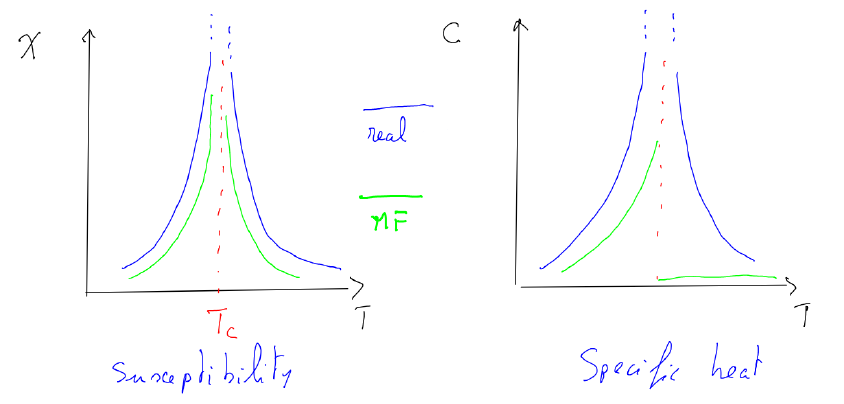
\includegraphics[width=0.9\textwidth]{chi-cv.png}
    \caption{Plot of the susceptibility $\chi$ (left) and the specific heat per node $c$ (right) as functions of temperature $T$. Both quantities \textit{diverge} for $T \to T_c$ in the real case - but this behaviour is captured by the mean field approximation only for $\chi$, and not for $c$ - for which only a \textit{finite} jump discontinuity is predicted. Even in the case of $\chi$, in a real system it diverges more rapidly than in the mean field model.}
    \label{fig:chi-cv}
\end{figure}

\subsection{The scaling ansatz}
We can use the power laws we have just found to write an \textbf{equation of state} connecting $h$, $m$ and $t$ (temperature difference to criticality). 

\medskip

We start from (\ref{eqn:h-eq}), highlight a $t$ and collect a $m^3$:
\begin{align*}
    h = m^3 \Bigg[\frac{1}{3} + \overbrace{\frac{K_c - K}{K_c}}^{t}m^{-2} + O(m^2) \Bigg] \qquad K \sim K_c;\> h\sim 0
\end{align*}
As in the mean-field $\beta = 1/2$ (\ref{eqn:m-power-law-h0}), we can rewrite $m^{-2} = m^{-1/\beta}$. We then use (\ref{eqn:m-power-law-h}) to write $m^3 = m|m|^{\delta-1}$, leading to the \textbf{scaling ansatz}, first conjectured by Widom in 1960:
\begin{align}\label{eqn:h-equation-state}
    h = m|m|^{\delta -1} h_s(t|m|^{-1/\beta}) \qquad  \quad t = \frac{T-T_c}{T_c}  
\end{align}
Where $h_s$ (the \q{scaling function}), has the following form in the mean field approximation:
\begin{align*}
    h_s(x) = \frac{1}{3} + x
\end{align*}
It is conjectured that, in general, $h_s$ will be a increasing function of the argument, becoming $0$ at a \textit{negative} value of the argument (fig. \ref{fig:scaling-function}).

\begin{figure}[H]
    \centering
    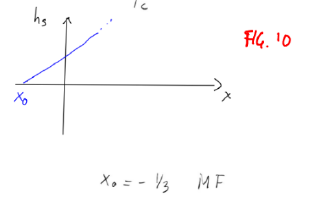
\includegraphics[width=0.7\textwidth]{scaling-function.png}
    \caption{Plot of the scaling function $h_S$ for the Mean Field case.}
    \label{fig:scaling-function}
\end{figure}

Equation (\ref{eqn:h-equation-state}) summarizes the previous scaling laws, in particular (\ref{eqn:m-power-law-h0}), (\ref{eqn:m-power-law-h}) and (\ref{eqn:susceptibility-power-law}) in all cases ($h=0$ or $h\neq 0$, $T < T_c$ or $T > T_c$). So, in the hypothesis that an equation of state of the form (\ref{eqn:h-equation-state}) holds in a more general case, and not only in the mean field approximation (eventually with different values for the exponent), we have a way to re-derive scaling laws in a more general case.

\medskip

Explicitly, assuming $h_S$ monotonically increasing with $h_S(x_0) = 0$ and $x_0 < 0$:
\begin{enumerate}
    \item \textbf{Magnetization}. If $h=0$, equation (\ref{eqn:h-equation-state}) becomes:
    \begin{align*}
        0 = m|m|^{\delta-1} h_s(t|m|^{-1/\beta})
    \end{align*}
    The possible solutions are $m=0$ or $t|m|^{-1/\beta} = x_0 < 0$. However, the second one is present only if $t < 0$, and so:
    \begin{align*}
        m = \begin{cases}
            0 & t < 0\\
            (-t)^\beta |x_0| & t > 0
        \end{cases}
    \end{align*} %TODO Verify
    \item \textbf{Susceptibility}. Differentiating (\ref{eqn:h-equation-state}) with respect to $m$ and evaluating at $h=0$ leads to:
    \begin{align*}
        \chi^{-1} = \pdv{h}{m}\Big|_{h=0} = |m|^{\delta-1}\left[\delta h_S(x) - \frac{x}{\beta} h_S'(x) \right]_{h=0}
    \end{align*} %TODO complete (from pag. 20)
\end{enumerate}

In essence, the scaling ansatz (\ref{eqn:h-equation-state}) comes from the peculiar scaling of $m$ in a neighbourhood of criticality (fig. \ref{fig:criticality-vicinity}), and in particular: 
\begin{enumerate}[label=\alph*)]
    \item \label{item:1} For $h=0$ fixed and $t = (T-T_c)/T_c \approx 0$ (i.e. varying in the vicinity of the critical point), $m \propto (-t)^\beta$ for $t \lesssim 0$.
    \item \label{item:2} For $t=0$ fixed and $h$ varying, $|m| \propto |h|^{1/\delta}$.
\end{enumerate} %TODO Add references

\begin{figure}[H]
    \centering
    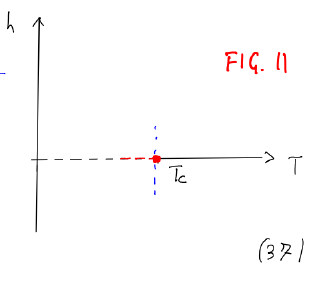
\includegraphics[width=0.6\textwidth]{criticality-vicinity.png}
    \caption{Phase diagram in $h$ and $T$. Singularities of $F_V$ are represented as the black dots at the left of $T_c$. The scaling ansatz describes how $m$ changes when approaching the critical point \textit{horizontally} (along the red path), i.e. at $h=0$ and varying $T$, or \textit{vertically}, i.e. at $T = T_c$ and varying $h$.}
    \label{fig:criticality-vicinity}
\end{figure}

In principle it is natural to say that $h$ should depend on two independent variables - $t$ and $m$ - but the choice of the \textit{form} of (\ref{eqn:h-equation-state}) arises from some \textbf{non-trivial} dimensional analysis arguments. The idea comes from observing that certain \textit{ratios} of quantities - due to their scaling behaviour near criticality (\ref{item:1} and \ref{item:2}) - are \q{dimensionless}\footnote{Not in the sense that being \textit{pure numbers}, i.e. not having physical dimensions (e.g. $\si{\kilo\g}$, $\si{T}$, $\si{\K}$ etc.) - which is a matter of the so-called na\"ive dimensional analysis. The \q{non-trivial} dimensional analysis deals with \textit{scaling} and \textit{local behaviours}.}, in the sense that, near criticality, they \textit{do not depend} anymore on the distance from the critical point and are \q{devoid} of singularities. Some of them are $h/m|m|^{\delta-1}$, $t/|m|^{1/\beta}$ and $t|h|^{-1/\delta \beta}$ - and so (\ref{eqn:h-equation-state}) is written as a function of such arguments.


\begin{figure}[H]
    \centering
    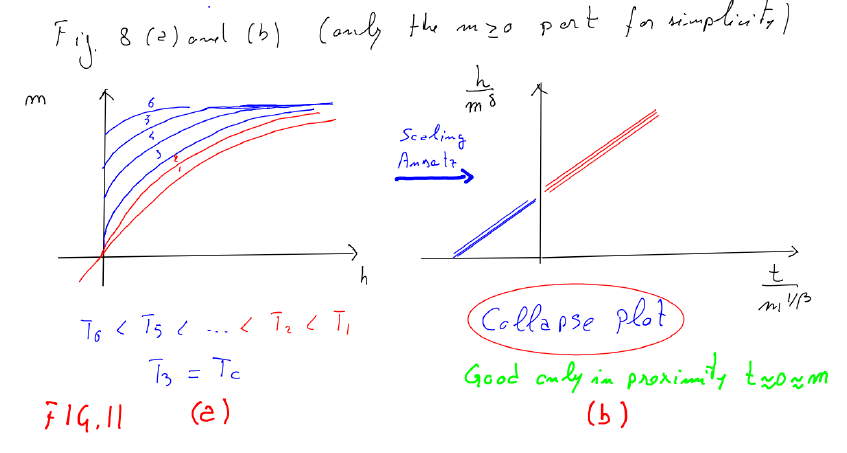
\includegraphics[width=0.9\textwidth]{collapse_plot.png}
    \caption{(a): $m(h)$ for different values of $K(T)$. When $T > T_c$ (hot system), $m(h)$ passes through the origin (red lines), while if $T < T_c$ (cold system), there is a nonzero spontaneous magnetization, i.e. $m(0) \neq 0$. As $m(h)$ is an odd function, only the first quadrant is shown for simplicity. If we instead plot \q{dimensionless} variables (b), all these curves \textit{collapse} into a single line (at least for $K(T)$ close to $K_c = K(T_c)$, i.e. $t \approx 0 \approx m$). This happens in the mean field approximation, and motivates a generalization to more complex systems giving rise to the scaling ansatz (\ref{eqn:h-equation-state}).}
    \label{fig:collapse_plot}
\end{figure}

\subsection{Two-point correlation function}
By shining a light on a fluid and measuring its scattering we can estimate how the density (and thus the refraction index) changes from point to point, and in particular its \textit{correlation} between different points. That's why it is important to compute correlation functions, especially the \textbf{two-point correlation} one:
\begin{align*}
    g(\bm{r}) \equiv \langle \sigma_x \sigma_y \rangle - \langle \sigma_x \rangle \langle \sigma_y \rangle
\end{align*} 
For the $d=1$ Ising model with $h=0$ and open boundary conditions we obtain:
\begin{align*}
    \langle \sigma_x \rangle &= 0\\
    \langle \sigma_x \sigma_y \rangle &= \sum_{\bm{\sigma}} \sigma_x \sigma_y \frac{1}{Z}  \exp\left(K \sum_z \sigma_z \sigma_{z+1}\right) =\\
    \shortintertext{Factoring the exponential over neighbouring pairs:}
    &= \sum_{\bm{\sigma}} \sigma_x \sigma_y \frac{1}{Z}  \prod_z \hlc{Yellow}{\exp\left(K \sigma_z \sigma_{z+1} \right)} =
    \shortintertext{As $\sigma_z \sigma_{z+1}$ is a binary variable (it can be only $\pm 1$), we can rewrite it using (\ref{eqn:ehsigma}, pag. \pageref{eqn:ehsigma}):}
    &= \sum_{\bm{\sigma}} \frac{\sigma_x \sigma_y}{Z}  \prod_z  (\cosh K + \sigma_z \sigma_{z+1} \sinh K)
    \shortintertext{Then we expand $Z = (2\cosh K)^N$ (\ref{eqn:Z-open-boundaries}, pag. \pageref{eqn:Z-open-boundaries}) and simplify the $\cosh K$:}
    &= \sum_{\bm{\sigma}} \sigma_x \sigma_y \frac{\prod_z \cosh K (1+ \sigma_z \sigma_{z+1} \tanh K)}{(2\cosh K)^L} = \\
    &= \sum_{\bm{\sigma}} \sigma_x \sigma_y \frac{\cancel{(\cosh K)^N} \prod_z (1+\sigma_z \sigma_{z+1} \tanh K)}{(2\cancel{\cosh K})^N} =\\
    &= %TODO Fix 2 factor
    \sum_{\bm{\sigma}} \sigma_x \sigma_y \prod_z (1 + \sigma_z \sigma_{z+1} \tanh K) =\\
    &= (\tanh K)^{|x-y|} %TODO Complete. Do it for N = 3 manually, and generalize from there (it should be "trivial" once understood) The only remaining term should be the one with only the sigma between x and y
\end{align*}
Thus the two-point correlation function can be written as:
\begin{align}\label{eqn:2point-exp-behaviour}
    g(r) = (\tanh K)^{|r|} = \exp\left(-\frac{|r|}{\xi(K)} \right)
\end{align}
where $\xi(K)$ is called the \textbf{correlation length}, and measures the \textit{decay} of correlations. In other words, spins are significantly correlated only when they are $|r| < \xi(K)$ positions apart. 

\medskip

Note that:
\begin{align*}
    \xi(K) = - \frac{1}{\ln \tanh K}  
\end{align*}
diverges when $K \to \infty$, i.e. when $T \to 0$. At very low temperature, the one-dimensional Ising model becomes \textit{fixed} in a extremely correlated configuration - as if $T=0$ were its the \textbf{critical temperature}. Still, note that this does not agree with the mean field model, for which $K_c = 1/2d = 1/2 \Rightarrow T_c = 2 J /k_B$. 

\medskip

The exponential behaviour of the two-point correlation function (\ref{eqn:2point-exp-behaviour}) motivates an \textit{ansatz} for models in $d \geq 2$. More precisely, when $t \neq 0$ (i.e. $T \neq T_c$) the two-point correlation function is suspected to have the form:
\begin{align*}
    g(\bm{r}, t) = r^{-\tau} \exp\left(-\frac{\tau}{\xi(t)} \right) \qquad r=\norm{\bm{r}}
\end{align*} 
with the correlation length diverging near the critical point:
\begin{align*}
    \xi(t) = C_\pm |t|^{-\nu} \qquad t \approx 0, \> h = 0
\end{align*}
for some proper choices of parameters $\tau$, $\nu$ and $C_\pm$. In more general cases, $\xi(t)$ may also depend (weakly) on the \textit{direction} of $\bm{r}$, meaning that the system is not isotropous.

\medskip

At the critical point %TODO 16.33 onwards

\end{document}
